\vspace{-1mm}
\section{Problemin A\c{c}{\i}klamas{\i}}
%
\begin{wrapfigure}{r}{0.4\textwidth} %this figure will be at the right
    \vspace{-5mm}
    \centering
    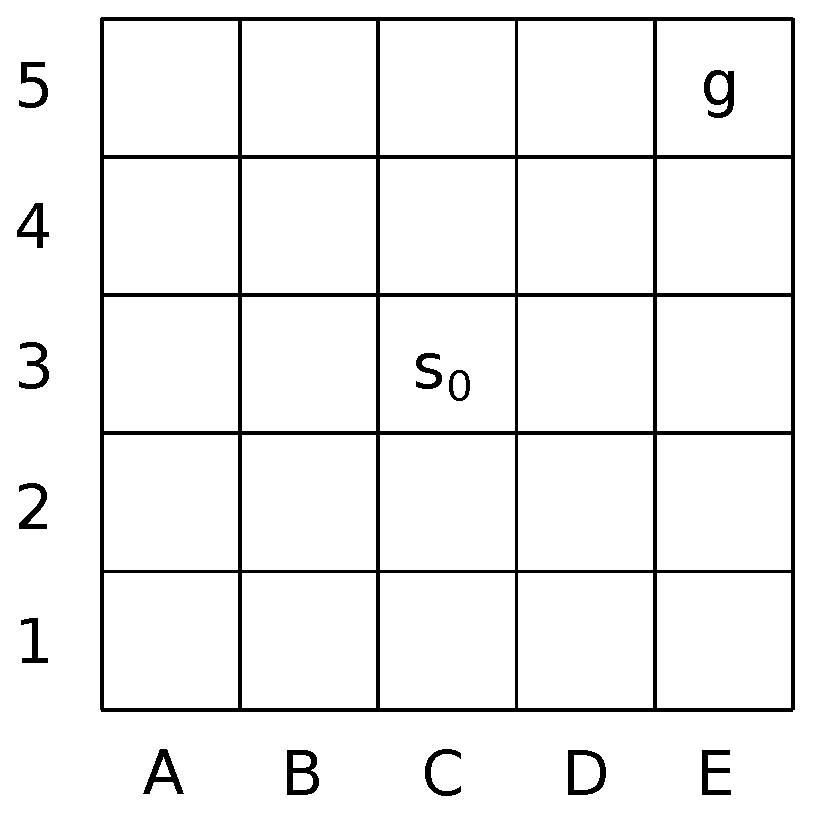
\includegraphics[width=0.25\textwidth]{./figures/drawing.eps}
    \caption{Problemin \c{s}emati\u{g}i}
    \label{fig:schematic}
    \vspace{-5mm}
\end{wrapfigure}
%
$5 \times 5$ bir satran\c{c} tahtas{\i} \"{u}st\"{u}ndeki karelerin yatayda A,
B, C, D, E, dikeyde ise 1, 2, 3, 4, 5 \c{s}eklinde kodland{\i}\u{g}{\i}n{\i} ve
C3 karesinde uzaktan kumandal{\i} bir robotunuz oldu\u{g}unu varsayal{\i}m.
Robotun kumandas{\i}n{\i}n robotu yukar{\i}, a\c{s}a\u{g}{\i}, sola veya
sa\u{g}a 1 kare hareket ettirecek \c{s}ekilde 4 tu\c{s}lu olarak
tasarland{\i}\u{g}{\i}n{\i}, fakat haylaz karde\c{s}inizin kumandan{\i}n
tu\c{s}lar{\i}n{\i}n yerlerini de\u{g}i\c{s}tirdi\u{g}ini d\"{u}\c{s}\"{u}nelim.
Tu\c{s}lar{\i} bir kere kar{\i}\c{s}t{\i}r{\i}l{\i}p sabitlenen kumanda ile
robotunuzu E5 noktas{\i}ndaki kareye g\"{o}t\"{u}rmek i\c{c}in basman{\i}z
gereken minimum tu\c{s} say{\i}s{\i}n{\i}n beklenen de\u{g}eri ka\c{c}t{\i}r?